%%%%%%%%%%%%%%%%%%%%%%%%%%%%%%%%%%%%%%%%%%%%%%%%%%%%%%%%%%%%%%%%%%%%%%%%%%%%%%%%
\chapter{Building graphs with a graph name}
\label{sec:Building-graphs-with-a-graph-name}
%%%%%%%%%%%%%%%%%%%%%%%%%%%%%%%%%%%%%%%%%%%%%%%%%%%%%%%%%%%%%%%%%%%%%%%%%%%%%%%%

Up until now, the graphs created have had no properties themselves.
Sure, the edges and vertices have had properties, but the graph itself
has had none.
Until now.

In this chapter, graphs will be created with a graph name of type std::string

\begin{itemize}
  \item An empty directed graph with a graph name: 
    see chapter 
  \item An empty undirected graph with a graph name: 
    see chapter 
  \item A two-state Markov chain with a graph name: 
    see chapter
  \item $K_{3}$ with a graph name: 
   see chapter 
\end{itemize}

In the process, some basic (sometimes bordering trivial) functions are shown:

\begin{itemize}
  \item Getting a graph its name: 
    see chapter 
  \item Setting a graph its name: 
    see chapter
\end{itemize}

%%%%%%%%%%%%%%%%%%%%%%%%%%%%%%%%%%%%%%%%%%%%%%%%%%%%%%%%%%%%%%%%%%%%%%%%%%%%%%%%
\section{Create an empty directed graph with a graph name property}
\label{subsec:create_empty_directed_graph_with_graph_name}
%%%%%%%%%%%%%%%%%%%%%%%%%%%%%%%%%%%%%%%%%%%%%%%%%%%%%%%%%%%%%%%%%%%%%%%%%%%%%%%%

Listing 
\ref{lst:create_empty_directed_graph_with_graph_name}
shows the function to create an empty directed graph with a graph name.

\lstinputlisting[
  caption = Creating an empty directed graph with a graph name,
  label = lst:create_empty_directed_graph_with_graph_name
]{create_empty_directed_graph_with_graph_name.impl}
\index{Create empty directed graph with graph name}

This \verb;boost::adjacency_list; is of the following type:

\begin{itemize}
  \item the first \verb;boost::vecS; \index{boost::vecS}: 
    select (that is what the \verb;S; \index{S} means) 
    that out edges are stored in a std::vector.
    This is the default way.
  \item the second \verb;boost::vecS; \index{boost::vecS}: 
    select that the graph vertices are stored in a std::vector.
    This is the default way.
  \item \verb;boost::directedS; \index{boost::directedS}: 
    select that the graph is directed.
    This is the default selectedness
  \item the first \verb;boost::no_property; \index{boost::no\_property}: 
    the vertices have no properties.
    This is the default (non-)property
  \item the second \verb;boost::no_property; \index{boost::no\_property}: 
    the vertices have no properties.
    This is the default (non-)property
  \item
    \verb;boost::property<boost::graph_name_t, std::string>; 
    \index{boost::property}
    \index{boost::graph\_name\_t}: 
    the graph itself has a single property: 
    its \verb;boost::graph_name; \index{boost::graph\_name} has type std::string
\end{itemize}

Listing 
\ref{lst:create_empty_directed_graph_with_graph_name_demo}
demonstrates the \verb;create_empty_directed_graph_with_graph_name; function.

\lstinputlisting[
  caption = Demonstration of create\_empty\_directed\_graph\_with\_graph\_name,
  label = lst:create_empty_directed_graph_with_graph_name_demo
]{create_empty_directed_graph_with_graph_name_demo.impl}

%%%%%%%%%%%%%%%%%%%%%%%%%%%%%%%%%%%%%%%%%%%%%%%%%%%%%%%%%%%%%%%%%%%%%%%%%%%%%%%%
\section{Create an empty undirected graph with a graph name property}
\label{subsec:create_empty_undirected_graph_with_graph_name}
%%%%%%%%%%%%%%%%%%%%%%%%%%%%%%%%%%%%%%%%%%%%%%%%%%%%%%%%%%%%%%%%%%%%%%%%%%%%%%%%

Listing 
\ref{lst:create_empty_undirected_graph_with_graph_name}
shows the function to create an empty undirected graph with a graph name.

\lstinputlisting[
  caption = Creating an empty undirected graph with a graph name,
  label = lst:create_empty_undirected_graph_with_graph_name
]{create_empty_undirected_graph_with_graph_name.impl}
\index{Create empty undirected graph with graph name}

This code is very similar to the code described in chapter 
\ref{lst:create_empty_directed_graph_with_graph_name}, 
except that the directness (the third template argument) is undirected
(due to the boost::undirectedS \index{boost::undirectedS}).

Listing \ref{lst:create_empty_undirected_graph_with_graph_name_demo}
demonstrates the \verb;create_empty_undirected_graph_with_graph_name; function.

\lstinputlisting[
  caption = Demonstration of create\_empty\_undirected\_graph\_with\_graph\_name,
  label = lst:create_empty_undirected_graph_with_graph_name_demo
]{create_empty_undirected_graph_with_graph_name_demo.impl}

%%%%%%%%%%%%%%%%%%%%%%%%%%%%%%%%%%%%%%%%%%%%%%%%%%%%%%%%%%%%%%%%%%%%%%%%%%%%%%%%
\section{Get a graph its name property}
\label{subsec:get_graph_name}
%%%%%%%%%%%%%%%%%%%%%%%%%%%%%%%%%%%%%%%%%%%%%%%%%%%%%%%%%%%%%%%%%%%%%%%%%%%%%%%%

\lstinputlisting[
  caption = Get a graph its name,
  label = lst:get_graph_name
]{get_graph_name.impl}
\index{Get graph name}

Listing \ref{lst:get_graph_name_demo}
demonstrates the \verb;get_graph_name; function.

\lstinputlisting[
  caption = Demonstration of get\_graph\_name,
  label = lst:get_graph_name_demo
]{get_graph_name_demo.impl}

%%%%%%%%%%%%%%%%%%%%%%%%%%%%%%%%%%%%%%%%%%%%%%%%%%%%%%%%%%%%%%%%%%%%%%%%%%%%%%%%
\section{Set a graph its name property}
\label{subsec:set_graph_name}
%%%%%%%%%%%%%%%%%%%%%%%%%%%%%%%%%%%%%%%%%%%%%%%%%%%%%%%%%%%%%%%%%%%%%%%%%%%%%%%%

\lstinputlisting[
  caption = Set a graph its name,
  label = lst:set_graph_name
]{set_graph_name.impl}
\index{Set graph name}

Listing \ref{lst:set_graph_name_demo}
 demonstrates the \verb;set_graph_name; function.

\lstinputlisting[
  caption = Demonstration of set\_graph\_name,
  label = lst:set_graph_name_demo
]{set_graph_name_demo.impl}

%%%%%%%%%%%%%%%%%%%%%%%%%%%%%%%%%%%%%%%%%%%%%%%%%%%%%%%%%%%%%%%%%%%%%%%%%%%%%%%%
\section{Create a directed graph with a graph name property}
\label{subsec:create_markov_chain_with_graph_name}
%%%%%%%%%%%%%%%%%%%%%%%%%%%%%%%%%%%%%%%%%%%%%%%%%%%%%%%%%%%%%%%%%%%%%%%%%%%%%%%%

\subsection{Graph}

See figure \ref{fig:markov_chain}.

\subsection{Function to create such a graph}

Listing \ref{lst:create_markov_chain_with_graph_name}
shows the function to create an empty directed graph with a graph name.

\lstinputlisting[
  caption = Creating a two-state Markov chain with a graph name,
  label = lst:create_markov_chain_with_graph_name
]{create_markov_chain_with_graph_name.impl}
\index{Create Markov chain with graph name}

\subsection{Creating such a graph}

Listing 
\ref{lst:create_markov_chain_with_graph_name_demo}
demonstrates the \verb;create_markov_chain_with_graph_name; function.

\lstinputlisting[
  caption = Demonstration of create\_markov\_chain\_with\_graph\_name,
  label = lst:create_markov_chain_with_graph_name_demo
]{create_markov_chain_with_graph_name_demo.impl}

\subsection{The .dot file produced}

%
% TODO
%
%\lstinputlisting[
%  caption = .dot file created from the create\_markov\_chain\_with\_graph\_name function (algorithm \ref{lst:create_markov_chain_with_graph_name}) converted from graph to .dot file using algorithm \ref{lst:save_graph_to_dot},
%  label = lst:create_markov_chain_with_graph_name.dot
%]{create_markov_chain_with_graph_name.dot}

\subsection{The .svg file produced}

\begin{figure}[!htbp]
  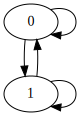
\includegraphics[]{create_markov_chain_with_graph_name.png}
  \caption{
    .svg file created from the create\_markov\_chain\_with\_graph\_name function 
    (algorithm \ref{lst:create_markov_chain_with_graph_name}) 
    its .dot file converted from .dot file to .svg 
    using algorithm \ref{lst:convert_dot_to_svg}
  }
  \label{fig:create_markov_chain_with_graph_name.svg}
\end{figure}

%%%%%%%%%%%%%%%%%%%%%%%%%%%%%%%%%%%%%%%%%%%%%%%%%%%%%%%%%%%%%%%%%%%%%%%%%%%%%%%%
\section{Create an undirected graph with a graph name property}
\label{subsec:create_k2_graph_with_graph_name}
%%%%%%%%%%%%%%%%%%%%%%%%%%%%%%%%%%%%%%%%%%%%%%%%%%%%%%%%%%%%%%%%%%%%%%%%%%%%%%%%

\subsection{Graph}

See figure \ref{fig:k2_graph}.

\subsection{Function to create such a graph}

Listing \ref{lst:create_k2_graph_with_graph_name}
shows the function to create K2 graph with a graph name.

\lstinputlisting[
  caption = Creating a K2 graph with a graph name,
  label = lst:create_k2_graph_with_graph_name
]{create_k2_graph_with_graph_name.impl}
\index{Create K2 graph with graph name}

\subsection{Creating such a graph}

Listing \ref{lst:create_k2_graph_with_graph_name_demo}
demonstrates the \verb;create_k2_graph_with_graph_name; function.

\lstinputlisting[
  caption = Demonstration of create\_k2\_graph\_with\_graph\_name,
  label = lst:create_k2_graph_with_graph_name_demo
]{create_k2_graph_with_graph_name_demo.impl}

\subsection{The .dot file produced}

\lstinputlisting[
  caption = .dot file created from the create\_k2\_graph\_with\_graph\_name function (algorithm \ref{lst:create_k2_graph_with_graph_name}) converted from graph to .dot file using algorithm \ref{lst:save_graph_to_dot},
  label = lst:create_k2_graph_with_graph_name.dot
]{create_k2_graph_with_graph_name.dot}

\subsection{The .svg file produced}

\begin{figure}[!htbp]
  \includegraphics[]{create_k2_graph_with_graph_name.png}
  \caption{
    .svg file created from the create\_k2\_graph\_with\_graph\_name function (algorithm
     \ref{lst:create_k2_graph_with_graph_name}) its .dot file, 
    converted from .dot file to .svg using algorithm 
    \ref{lst:convert_dot_to_svg}  
  }
  \label{fig:create_k2_graph_with_graph_name.svg}
\end{figure}

